\begin{table*}[t!]
  \small
  \begin{minipage}[t][9cm][t]{0.343\linewidth}
    \centering
    \captionsetup{justification=centering}
    \begin{minted}[xleftmargin=1em,linenos,autogobble,tabsize=2,framesep=1pt,frame=single,fontfamily=courier,fontsize=\fontsize{7}{8}\selectfont]{scala}
      //All networks have the same interface
      trait Network extends DFDesign {
        val iT = DFSInt[16] <> IN  //Top
        val iB = DFSInt[16] <> IN  //Bottom
        val oT = DFSInt[16] <> OUT //Top
        val oB = DFSInt[16] <> OUT //Bottom
      }
      //State in Top Connection
      trait NWLeft extends Network {
        iT.prev <> oT //Connection
        oB := iB * 3  //Assignment
      }
      //State in Bottom Assignment
      trait NWRight extends Network {
        iT <> oT + 5  //Connection
        oB := iB.prev //Assignment
      }
      //Parent box includes two sibling boxes
      trait NWParent extends Network {
        iT init (5, 7) //Initializing history
        iB init (2, 6) //Initializing history
        val nwL = new NWLeft {}
        val nwL = new NWRight {}
        nwL.iT <> iT
        nwL.iB <> iB
        nwR.oT <> oT
        nwR.oB <> oB
      }
      //Direct connections between siblings
      trait NWParDirect extends NWParent {
        nwL.oT <> nwR.iT
        nwL.oB <> nwR.iB
      }
      //Cross connections between siblings
      trait NWParCross extends NWParent {
        nwL.oT <> nwR.iB
        nwL.oB <> nwR.iT
      }
    \end{minted}
    \vfill
    \captionof{figure}{Various network designs \\ Featuring hierarchies and inheritance }
    \label{fig:BoxTopCode}
  \end{minipage}%
  \hfill
  \begin{minipage}[t][12cm][b]{0.64\linewidth}
    \centering
    \captionsetup{justification=centering}
    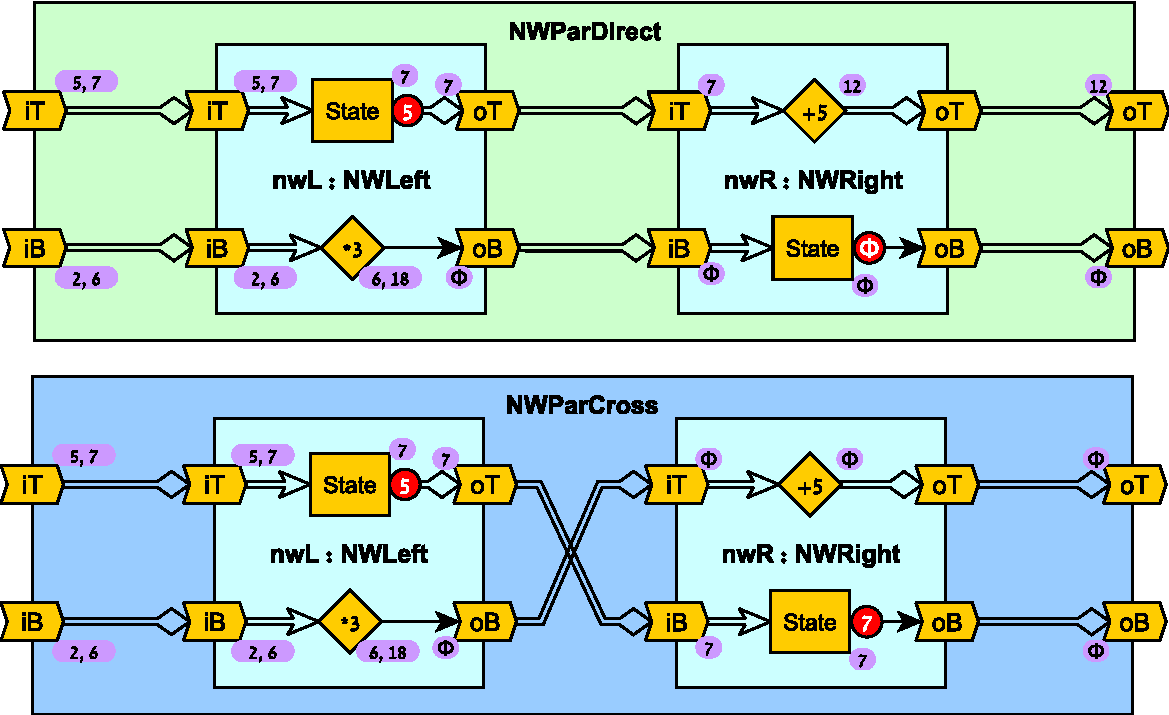
\includegraphics[width=0.9\linewidth]{graphics/connectivity.pdf}
    \captionof{figure}{
      Hierarichal drawing of \code{NWParDirect} and \code{NWParCross} \\
      The \colorbox{initcolor}{purple} numbers mark the initialization history as it is propagated according to the semantic rules of DFiant. The \colorbox{red}{\textcolor{white}{red}} numbers mark initial tokens generated by the state elements.
    }
    \vfill
    \label{fig:BoxTopDraw}
    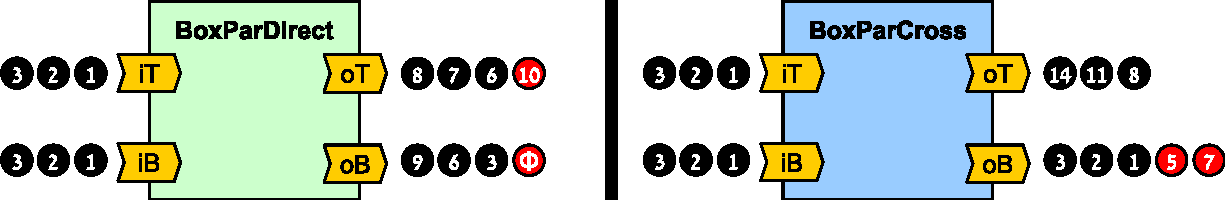
\includegraphics[width=0.9\linewidth]{graphics/connectivityTokens.pdf}
    \captionof{figure}{
      Input/Output token flow example to/from the two parent boxes (the rightmost tokens are the oldest). 
    }
    \label{fig:BoxTopTokens}
  \end{minipage}%
  \vspace{2ex}
  \hrule
  \vspace{2ex}
  \captionof{table}{Connection \code{<>} and Assignment \code{:=} Operator Comparison}
  \label{tbl:Box}
  \begin{tabular}{|c|c|c|}
    \hline 
    \textbf{Criteria} & \textbf{Connection \code{<>}} & \textbf{Assignment \code{:=}} \\ 
    \hline
    \begin{minipage}{0.1\textwidth}
      \flushleft
      Code
    \end{minipage} 
    &
    \begin{minipage}[c][1.5cm]{0.4\textwidth}
      \begin{minted}[autogobble,tabsize=2,framesep=1pt,fontfamily=pcr,fontsize=\fontsize{7}{8}\selectfont]{scala}
      trait IOConnection extends DFDesign {
        val i = DFUInt[8] <> IN
        val o = DFUInt[8] <> OUT
        o <> i
      }
      \end{minted}
    \end{minipage} 
    &  
    \begin{minipage}[c][1.5cm]{0.4\textwidth}
      \begin{minted}[autogobble,tabsize=2,framesep=1pt,fontfamily=pcr,fontsize=\fontsize{7}{8}\selectfont]{scala}
        trait IOAssignment extends DFDesign {
          val i = DFUInt[8] <> IN
          val o = DFUInt[8] <> OUT
          o := i
        }
      \end{minted}
    \end{minipage} 
    \\ 
    \hline 
    \begin{minipage}{0.1\textwidth}
      \flushleft
      Functional Diagram
    \end{minipage} 
    &
    \begin{minipage}[c][2cm]{0.10\textwidth}
      \centering
      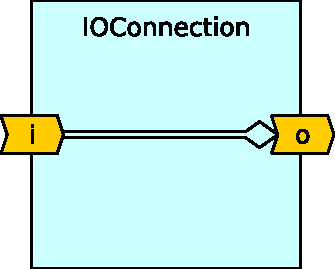
\includegraphics[height=1.8cm]{graphics/IOConnection.pdf}\\
    \end{minipage}%
    \hfill 
    \begin{minipage}[c][2cm]{0.27\textwidth}
      A double line arrow indicates a dataflow dependency \textbf{with} an initial condition dependency.
    \end{minipage} 
    &  
    \begin{minipage}[c][2cm]{0.10\textwidth}
      \centering
      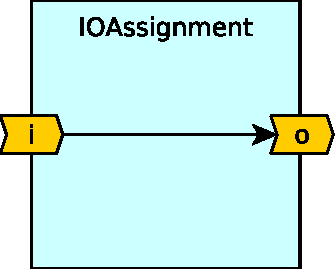
\includegraphics[height=1.8cm]{graphics/IOAssignment.pdf}\\
    \end{minipage}%
    \hfill 
    \begin{minipage}[c][2cm]{0.27\textwidth}
      A single line arrow indicates a dataflow dependency \textbf{without} affecting initial conditions of the consumer.
    \end{minipage} 
    \\ 
    \hline
    \begin{minipage}{0.1\textwidth}
      \flushleft
      Directionality \\and\\ Commutativity
    \end{minipage} 
    &
    \begin{minipage}[c][1.5cm]{0.42\textwidth}
      The operator is commutative, meaning \code{a <> b} is equivalent to \code{b <> a}. One argument is the \emph{producer}, while the other is the \emph{consumer}. The dataflow direction is sensitive to the context in which the operator is applied.
    \end{minipage} 
    &  
    \begin{minipage}[c][1.5cm]{0.42\textwidth}
      The operator is non-commutative, meaning \code{a := b} determines that \code{b} is the \emph{producer}, transferring data to the \emph{consumer} \code{a}.
    \end{minipage} 
    \\ 
    \hline
    \begin{minipage}{0.1\textwidth}
      Initialization
    \end{minipage} 
    &
    \begin{minipage}[c][1.2cm]{0.42\textwidth}
      Initialization is transferred to the consumer. If the consumer has both initialization via \code{.init} and connection, then the \code{.init} is the one that takes effect.
    \end{minipage} 
    &  
    \begin{minipage}[c][1.2cm]{0.42\textwidth}
      The consumer initialization is \textbf{not} affected.
    \end{minipage} 
    \\ 
    \hline
    \begin{minipage}{0.1\textwidth}
      \flushleft
      Mutation
    \end{minipage} 
    &
    \begin{minipage}[c][0.5cm]{0.42\textwidth}
      A consumer can only be connected once at each bit.
    \end{minipage} 
    &  
    \begin{minipage}[c][0.5cm]{0.42\textwidth}
      The same bit in a consumer can be assigned to more than once.
    \end{minipage} 
    \\ 
    \hline
    \begin{minipage}{0.1\textwidth}
      \flushleft
      Statement Order
    \end{minipage} 
    &
    \begin{minipage}[c][0.8cm]{0.42\textwidth}
      Connections statements can be placed in any order. 
      %Comment about versioning? About forbidding connections and assignments?
    \end{minipage} 
    &  
    \begin{minipage}[c][0.8cm]{0.42\textwidth}
      Assignments affect the scope reference of the modified dataflow variable, and therefore their order is highly important.
    \end{minipage}% 
    \\ 
    \hline
  \end{tabular}% 
\end{table*}
